\documentclass[10pt, aspectratio=169]{beamer}

% --- Configuración de Tema ---
\usetheme{Madrid}
\usecolortheme{beaver}
\usefonttheme{professionalfonts}
\usepackage[spanish]{babel}
\usepackage[utf8]{inputenc}
\usepackage{amsmath}
\usepackage{amsfonts}
\usepackage{amssymb}
\usepackage{graphicx}
\usepackage{booktabs}
\usepackage{xcolor}
\usepackage{colortbl}
\usepackage{caption}   % habilita \caption* sin prefijo "Figura:"
\usepackage{tikz}      % para logo arriba a la derecha

% --- Paleta de colores FIUBA ---
\definecolor{fiubablue}{RGB}{0,70,127}
\definecolor{fiubared}{RGB}{180,30,30}

\setbeamercolor{frametitle}{bg=fiubablue, fg=white}
\setbeamercolor{title}{fg=fiubablue}
\setbeamercolor{structure}{fg=fiubablue}
\setbeamercolor{block title}{bg=fiubablue, fg=white}
\setbeamercolor{block body}{bg=fiubablue!10}

% Ruta de figuras (el .tex está en ppt/, las figuras en Figures/)
\graphicspath{{../Figures/}}

% --- Logo arriba a la derecha en cada slide (excepto portada) ---
\addtobeamertemplate{frametitle}{}{%
  \begin{tikzpicture}[remember picture, overlay]
    \node[anchor=north east, xshift=-4pt, yshift=2pt]
      at (current page.north east)
      {\includegraphics[height=0.65cm]{logoFIUBA.pdf}};
  \end{tikzpicture}%
}

% --- Información de la Tesis ---
\title[Optimización biomecánica con IA]{Optimización biomecánica del ciclismo\\asistida por inteligencia artificial}
\author[Ing. Rodrigo Goñi]{Ing. Rodrigo Iván Goñi}
\institute[FIUBA]{
    Trabajo Final - Carrera de Especialización en Inteligencia Artificial}
\date[2026]{Ciudad de Mendoza, 2026}
\titlegraphic{\includegraphics[height=1.2cm]{logoFIUBA.pdf}}

\begin{document}

% ============================================================
% PORTADA
% ============================================================
\begin{frame}[plain]
    \titlepage
    \begin{center}
        \footnotesize
        \textbf{Director:} MSc. Fernando Corteggiano \\[2pt]
        \textbf{Jurados:} Dr. Ing. David Marcelo De Yong \quad
                          Esp. Ing. Fernando Monzón \quad
                          Ing. Octavio Deshays
    \end{center}
\end{frame}

% ============================================================
\section{Cap. 1 -- Introducción y contexto}
% ============================================================

% --- Contexto (problema_ajuste.jpg 1.73x WIDE -> columna derecha 55%) ---
\begin{frame}{Contexto y problemática}
    \begin{columns}[T]
        \begin{column}{0.42\textwidth}
            \begin{itemize}
                \item Biomecánica: factor clave para rendimiento y prevención de lesiones.
                \item Ajuste incorrecto $\Rightarrow$ hasta \textbf{20\,\%} menos de potencia.
                \item Soluciones profesionales: costosas, escasas y presenciales.
            \end{itemize}
        \end{column}
        \begin{column}{0.55\textwidth}
            \centering
            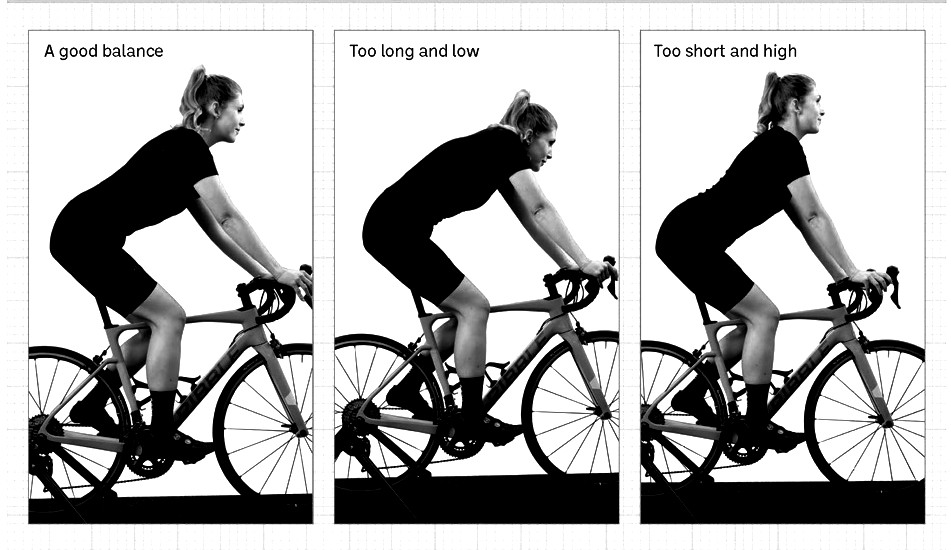
\includegraphics[width=\textwidth]{problema_ajuste.jpg}\\
            {\scriptsize Ejemplo de mal ajuste biomecánico.}
        \end{column}
    \end{columns}
\end{frame}

% --- Estado del Arte (modern_bikefitting.jpeg 1.32x -> columna derecha 50%) ---
\begin{frame}{Estado del arte}
    \begin{columns}[T]
        \begin{column}{0.47\textwidth}
            \begin{itemize}
                \item \textbf{Laboratorios 3D/4D:} cámaras infrarrojas (Retül, Vicon),
                      análisis dinámico multiplanar.
                \item \textbf{Aerodinámica:} CFD + IA para estimar $C_d A$.
                \item \textbf{Apps Móviles (2D):} mayor acceso, menor precisión
                      por error de perspectiva.
            \end{itemize}
        \end{column}
        \begin{column}{0.50\textwidth}
            \centering
            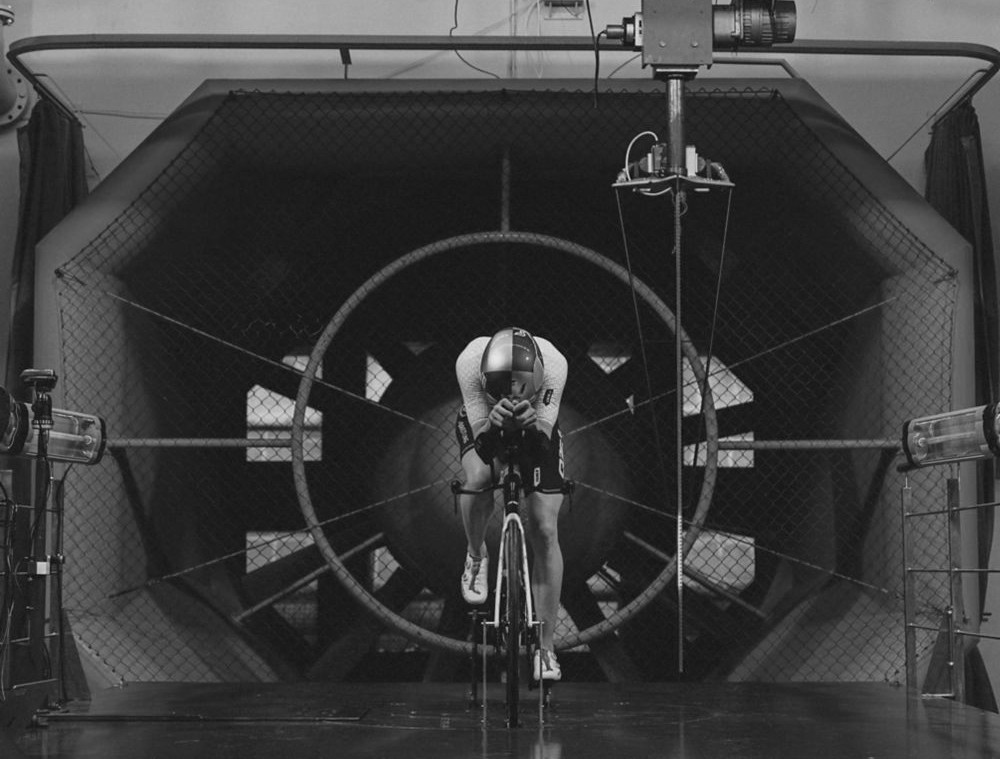
\includegraphics[width=\textwidth]{modern_bikefitting.jpeg}\\
            {\scriptsize Sistema profesional de \textit{bike fitting} en laboratorio.}
        \end{column}
    \end{columns}
\end{frame}

% --- Motivación (sin figura, bloques) ---
\begin{frame}{Motivación y objetivos}
    \begin{block}{Motivación}
        El ajuste biomecánico debe ser \textbf{dinámico y continuo},
        adaptándose a la evolución física del ciclista.
    \end{block}
    \vspace{4pt}
    \begin{block}{Objetivo principal}
        Desarrollar un \textbf{prototipo inteligente} para optimizar parámetros
        biomecánicos mediante visión artificial, modelado físico y optimización multi-objetivo.
    \end{block}
    \vspace{4pt}
    \begin{alertblock}{Compromiso de diseño}
        Maximizar potencia \quad|\quad Minimizar riesgo de lesiones \quad|\quad
        Equilibrar aerodinámica
    \end{alertblock}
\end{frame}

% ============================================================
\section{Cap. 2 -- Marco teórico}
% ============================================================

% --- BlazePose (pose_inferencia.png 0.91x CUADRADA -> columna lateral) ---
\begin{frame}{Estimación de pose: MediaPipe BlazePose}
    \begin{columns}[T]
        \begin{column}{0.50\textwidth}
            \begin{itemize}
                \item CNN con \textbf{33 landmarks}, incluyendo pies y talones.
                \item Filtro Prior Cinemático: corrige por invarianza de longitud de segmento óseo.
                \item Seleccionado por cobertura anatómica y velocidad de inferencia.
            \end{itemize}
        \end{column}
        \begin{column}{0.47\textwidth}
            \centering
            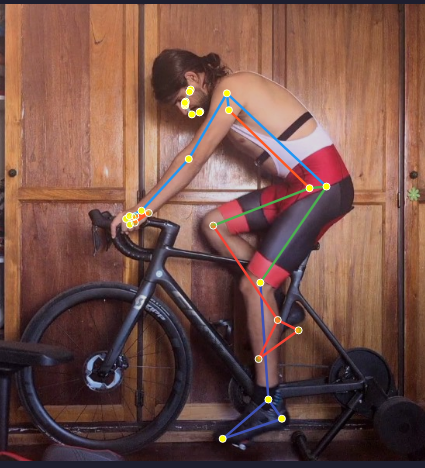
\includegraphics[width=0.82\textwidth]{pose_inferencia.png}\\
            {\scriptsize Inferencia de pose sobre el ciclista (MediaPipe BlazePose).}
        \end{column}
    \end{columns}
\end{frame}

% --- NSGA-II (evol_solv_ag.png 2.82x MUY ANCHA -> ancho completo abajo) ---
\begin{frame}{Optimización multi-objetivo: NSGA-II}
    \begin{itemize}
        \item \textbf{Variables} ($x \in \mathbb{R}^4$): altura/retroceso del sillín,
              altura/alcance del manillar.
        \item Codificación real, robusto ante no convexidad, ruido y discontinuidades.
    \end{itemize}
    \vspace{4pt}
    \centering
    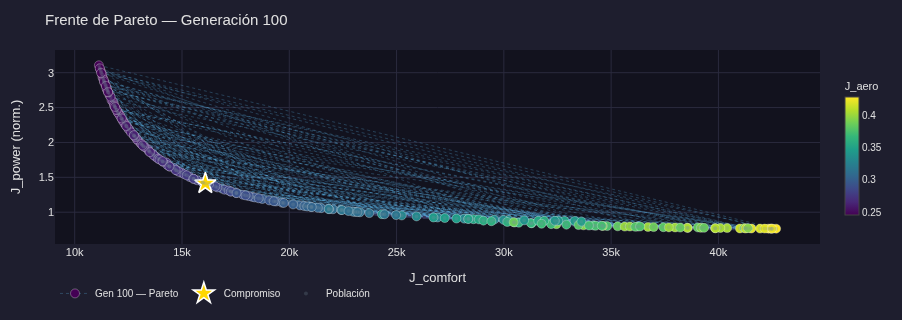
\includegraphics[width=\textwidth]{evol_solv_ag.png}\\
    {\scriptsize Evolución del frente de Pareto por generación.}
\end{frame}

% ============================================================
\section{Cap. 3 -- Diseño e implementación}
% ============================================================

% --- CRISP-DM: solo diagrama centrado ---
\begin{frame}{Metodología CRISP-DM adaptada}
    \vspace{-4pt}
    \begin{center}
        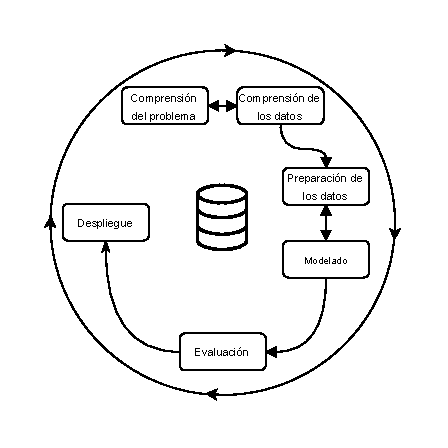
\includegraphics[width=0.70\textwidth, height=0.74\textheight, keepaspectratio]{crispdm.pdf}
    \end{center}
    \vspace{2pt}
    {\centering\scriptsize Metodología CRISP-DM adaptada al dominio biomecánico.\par}
\end{frame}

% --- Arquitectura: PNG a ancho completo (1.79x WIDE) ---
\begin{frame}{Arquitectura del pipeline}
    \vspace{-6pt}
    \begin{center}
        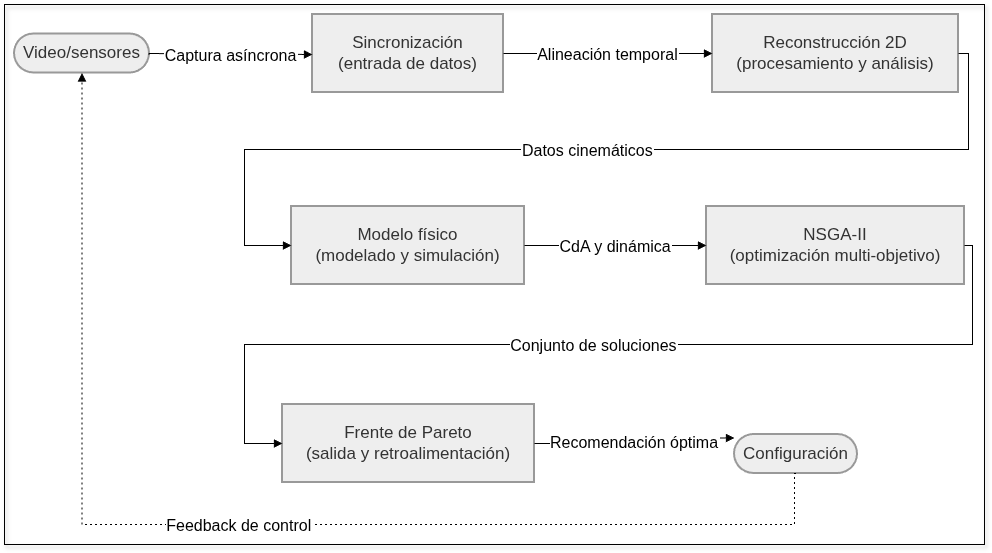
\includegraphics[width=0.9\textwidth, height=0.78\textheight, keepaspectratio]{Arquitectura_Pipeline.png}
    \end{center}
    \vspace{-4pt}
    {\centering\scriptsize Flujo multimodal: adquisición $\to$ percepción $\to$ modelado físico $\to$ optimización NSGA-II $\to$ reporte.\par}
\end{frame}

% --- Adquisición (calidad_pixel8pro.png 0.89x CUADRADA -> columna lateral) ---
\begin{frame}{Adquisición de datos y sincronización}
    \begin{columns}[T]
        \begin{column}{0.53\textwidth}
            \begin{itemize}
                \item LifeCam: \textit{motion blur} inaceptable.
                \item \textbf{Pixel\,8\,Pro}: exposición $\le 1/500$\,s,
                      $\ge 60$\,FPS.
                \item Sincronización A/V: correlación cruzada normalizada
                      cadencia visual--rodillo.
                \item Calibración métrica: rueda 700c (622\,mm).
            \end{itemize}
        \end{column}
        \begin{column}{0.44\textwidth}
            \centering
            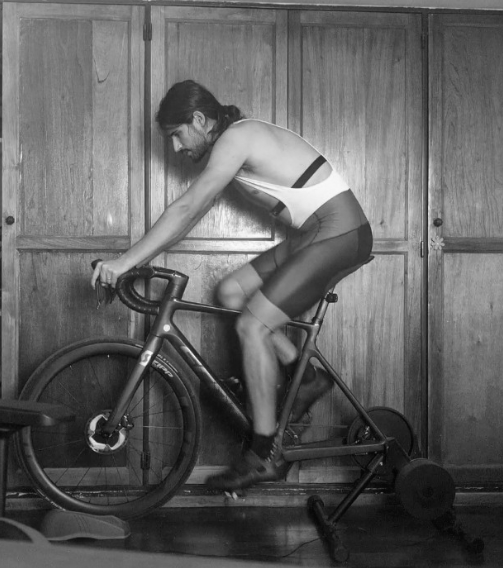
\includegraphics[width=\textwidth]{calidad_pixel8pro.png}\\
            {\scriptsize Calidad de captura con Pixel\,8\,Pro.}
        \end{column}
    \end{columns}
\end{frame}

% --- Kalman: solo una gráfica, máximo espacio ---
\begin{frame}{Modelado cinemático: filtro de Kalman}
    \vspace{-4pt}
    \begin{center}
        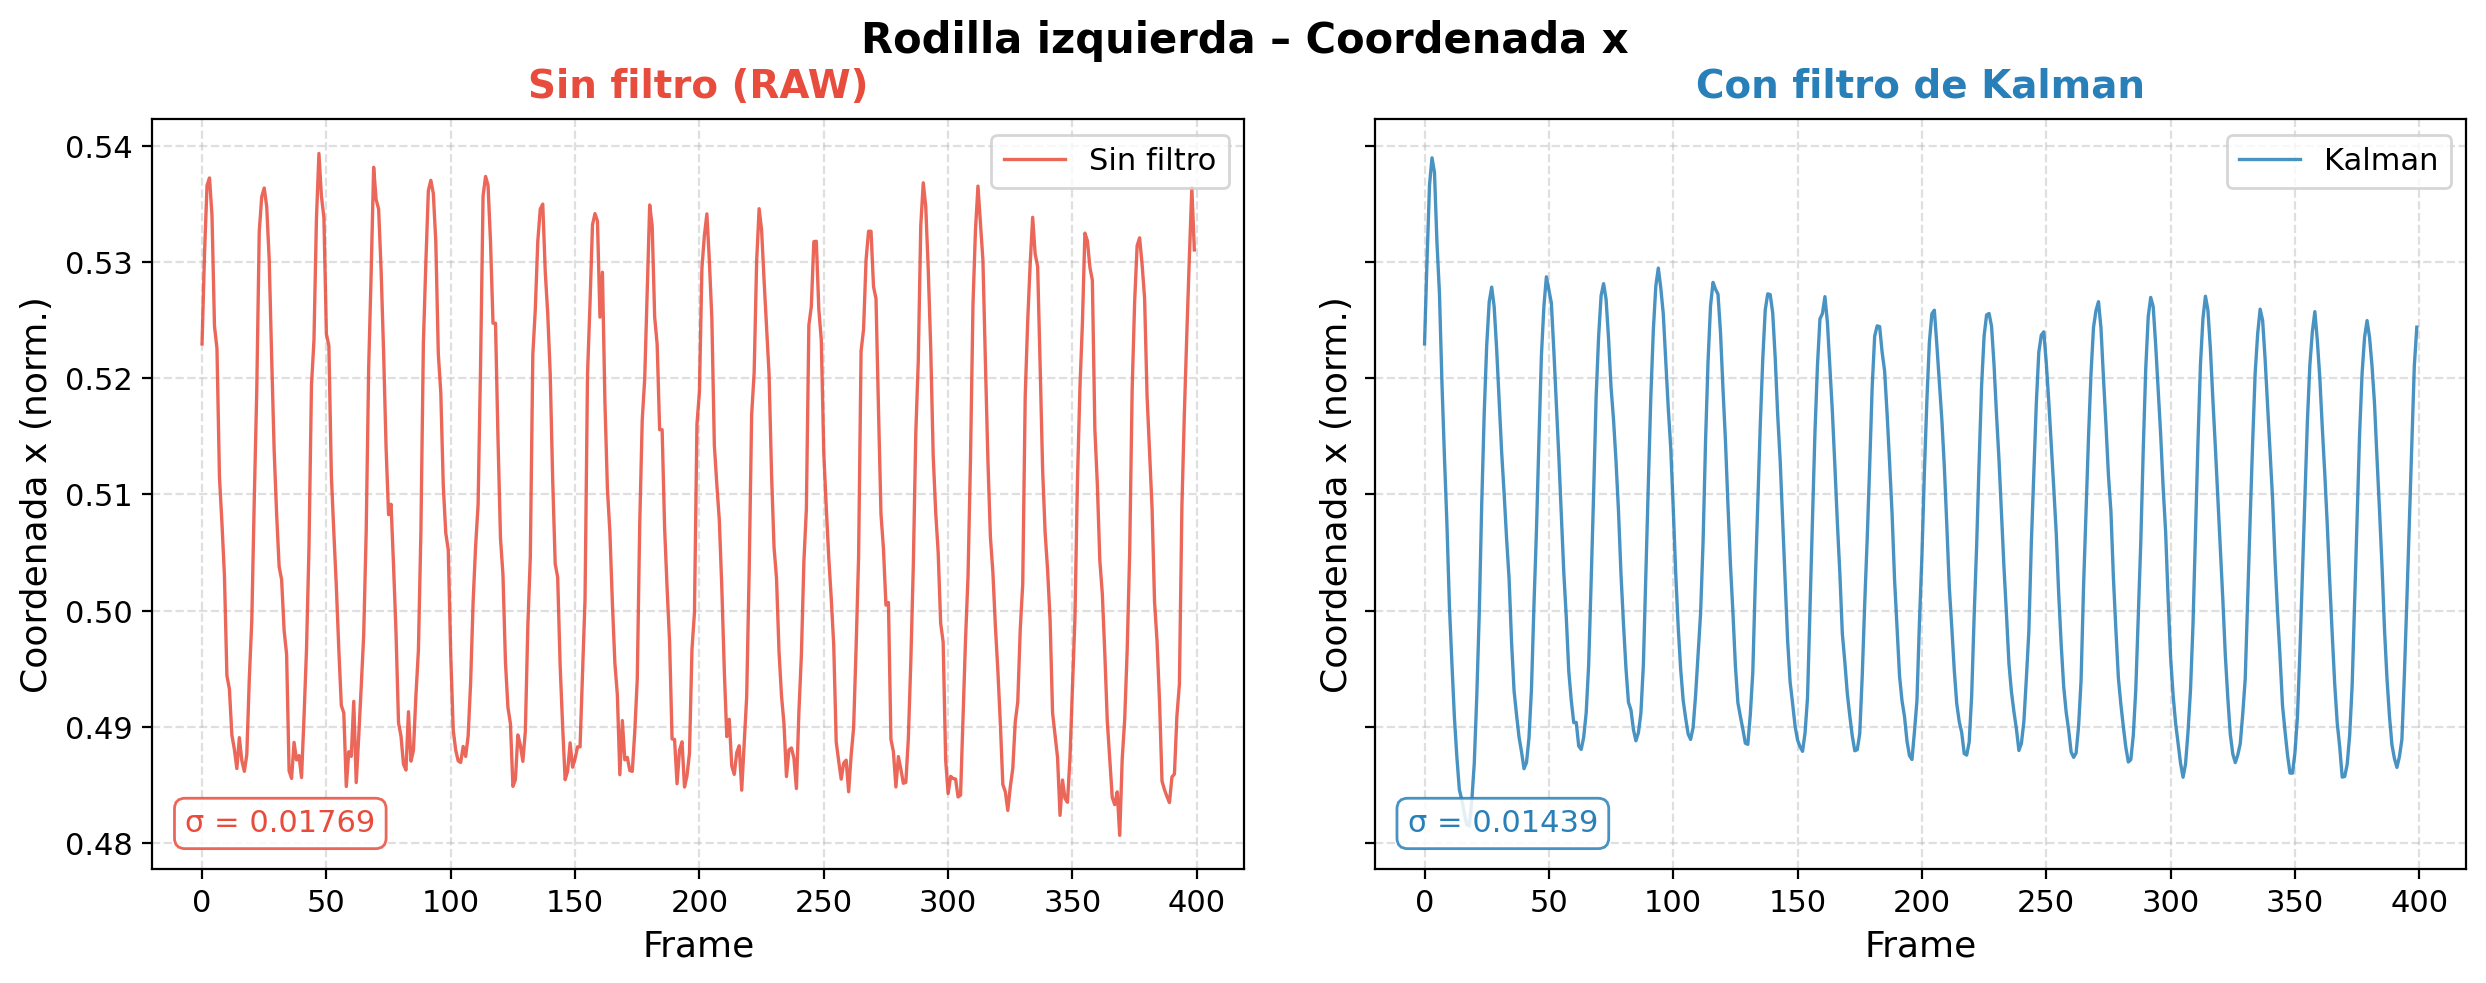
\includegraphics[width=\textwidth, height=0.80\textheight, keepaspectratio]{kalman_knee_x.png}
    \end{center}
    \vspace{-4pt}
    {\centering\scriptsize Señal RAW vs.\ Kalman de la coordenada $x$ de la rodilla. El filtro elimina el \textit{jitter} de BlazePose sin introducir latencia de fase apreciable.\par}
\end{frame}

% --- Dinámica inversa (fuerzas_frame.png 0.95x CUADRADA -> columna lateral) ---
\begin{frame}{Dinámica inversa y gemelo digital}
    \begin{columns}[T]
        \begin{column}{0.57\textwidth}
            \begin{itemize}
                \item Newton-Euler recursivo: pedal $\to$ tobillo $\to$ rodilla $\to$ cadera.
                \item Potencia articular:
                      $P = M_{joint}\cdot(\dot\theta_{prox} - \dot\theta_{dist})$
                \item Estimación de $C_d A$ sin túnel de viento
                      (modelo Heil + Bassett).
            \end{itemize}
        \end{column}
        \begin{column}{0.40\textwidth}
            \centering
            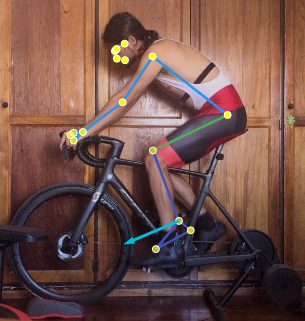
\includegraphics[width=0.85\textwidth]{fuerzas_frame.png}\\
            {\scriptsize Fuerzas en el pedal -- gemelo digital 2D.}
        \end{column}
    \end{columns}
\end{frame}

% --- Funciones objetivo (sin figura, bloques compactos) ---
\begin{frame}{Funciones objetivo del optimizador}
    \begin{block}{$J_\text{comfort}$ -- Seguridad articular}
        Penalización cuadrática por desviación de rangos articulares seguros.
    \end{block}
    \vspace{3pt}
    \begin{block}{$J_\text{power}$ -- Eficiencia mecánica}
        Minimiza $\sum M_{joint}^2$. Promueve fibras musculares tipo~I.
    \end{block}
    \vspace{3pt}
    \begin{block}{$J_\text{aero}$ -- Aerodinámica}
        Minimiza $A_{proj}(\theta_{torso})$. Reduce resistencia al avance.
    \end{block}
\end{frame}

% ============================================================
\section{Cap. 4 -- Ensayos y resultados}
% ============================================================

% --- Protocolo (prueba_panteadaFC.png 1.17x CUADRADA -> columna lateral) ---
\begin{frame}{Protocolo de prueba y equipamiento}
    \begin{columns}[T]
        \begin{column}{0.50\textwidth}
            \begin{itemize}
                \item Rodillo inteligente + GoldenCheetah (ANT+).
                \item Video: DroidCam + Pixel\,8\,Pro.
                \item \textbf{Rampa}: 130\,W $\to$ 250\,W a 90\,RPM.
                \item Calibración: rueda 700c (622\,mm).
            \end{itemize}
        \end{column}
        \begin{column}{0.47\textwidth}
            \centering
            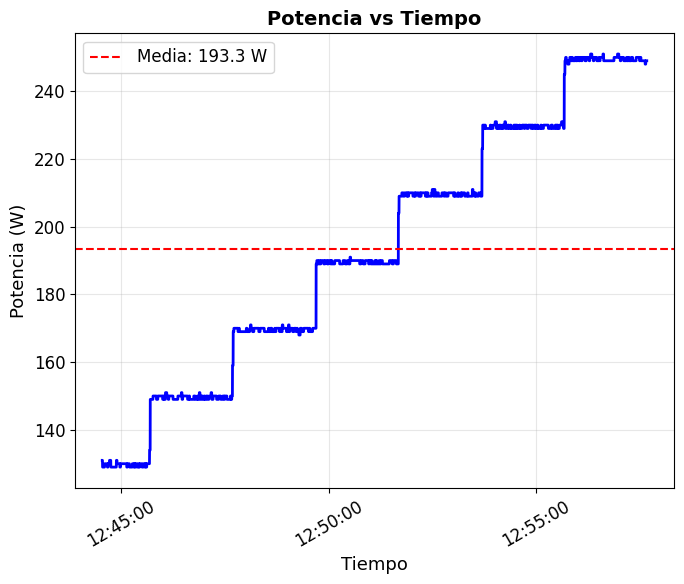
\includegraphics[width=\textwidth]{prueba_panteadaP.png}\\
            {\scriptsize Perfil de potencia durante el protocolo de rampa.}
        \end{column}
    \end{columns}
\end{frame}

% --- Interpolación: imagen correcta interpolacion_telemetria.png ---
\begin{frame}{Interpolación de telemetría}
    \vspace{-4pt}
    \begin{center}
        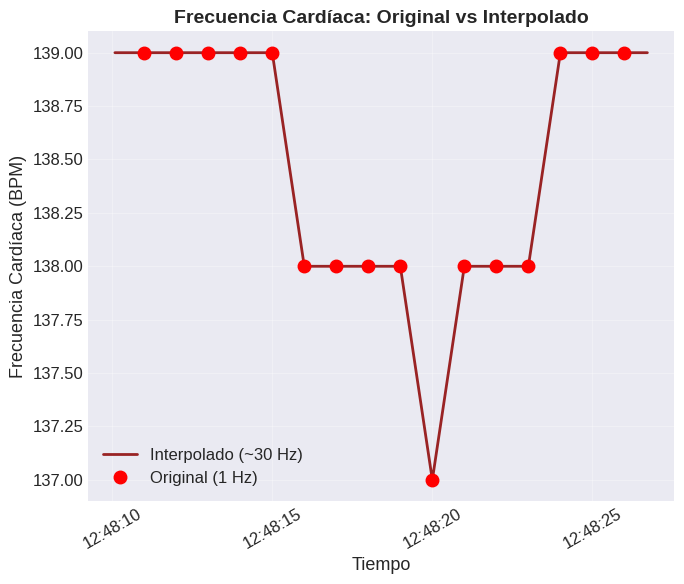
\includegraphics[width=0.80\textwidth, height=0.80\textheight, keepaspectratio]{interpolacion_telemetria.png}
    \end{center}
    \vspace{-4pt}
    {\centering\scriptsize Interpolación de señales telemetricas (1\,Hz $\to$ 30\,FPS) mediante \textit{spline} cúbico. Los escalones de potencia son claramente identificables.\par}
\end{frame}

% --- Pareto (pareto_nsga2_2d.png 1.26x CUADRADA -> imagen grande 62%) ---
\begin{frame}{Resultado: frontera de Pareto}
    \begin{columns}[T]
        \begin{column}{0.35\textwidth}
            \begin{itemize}
                \item Convergencia: \textbf{100 generaciones}.
                \item Solución de compromiso: mínima distancia euclídea normalizada
                      al origen.
                \item Balance objetivo entre confort, potencia y aerodinámica.
            \end{itemize}
        \end{column}
        \begin{column}{0.62\textwidth}
            \centering
            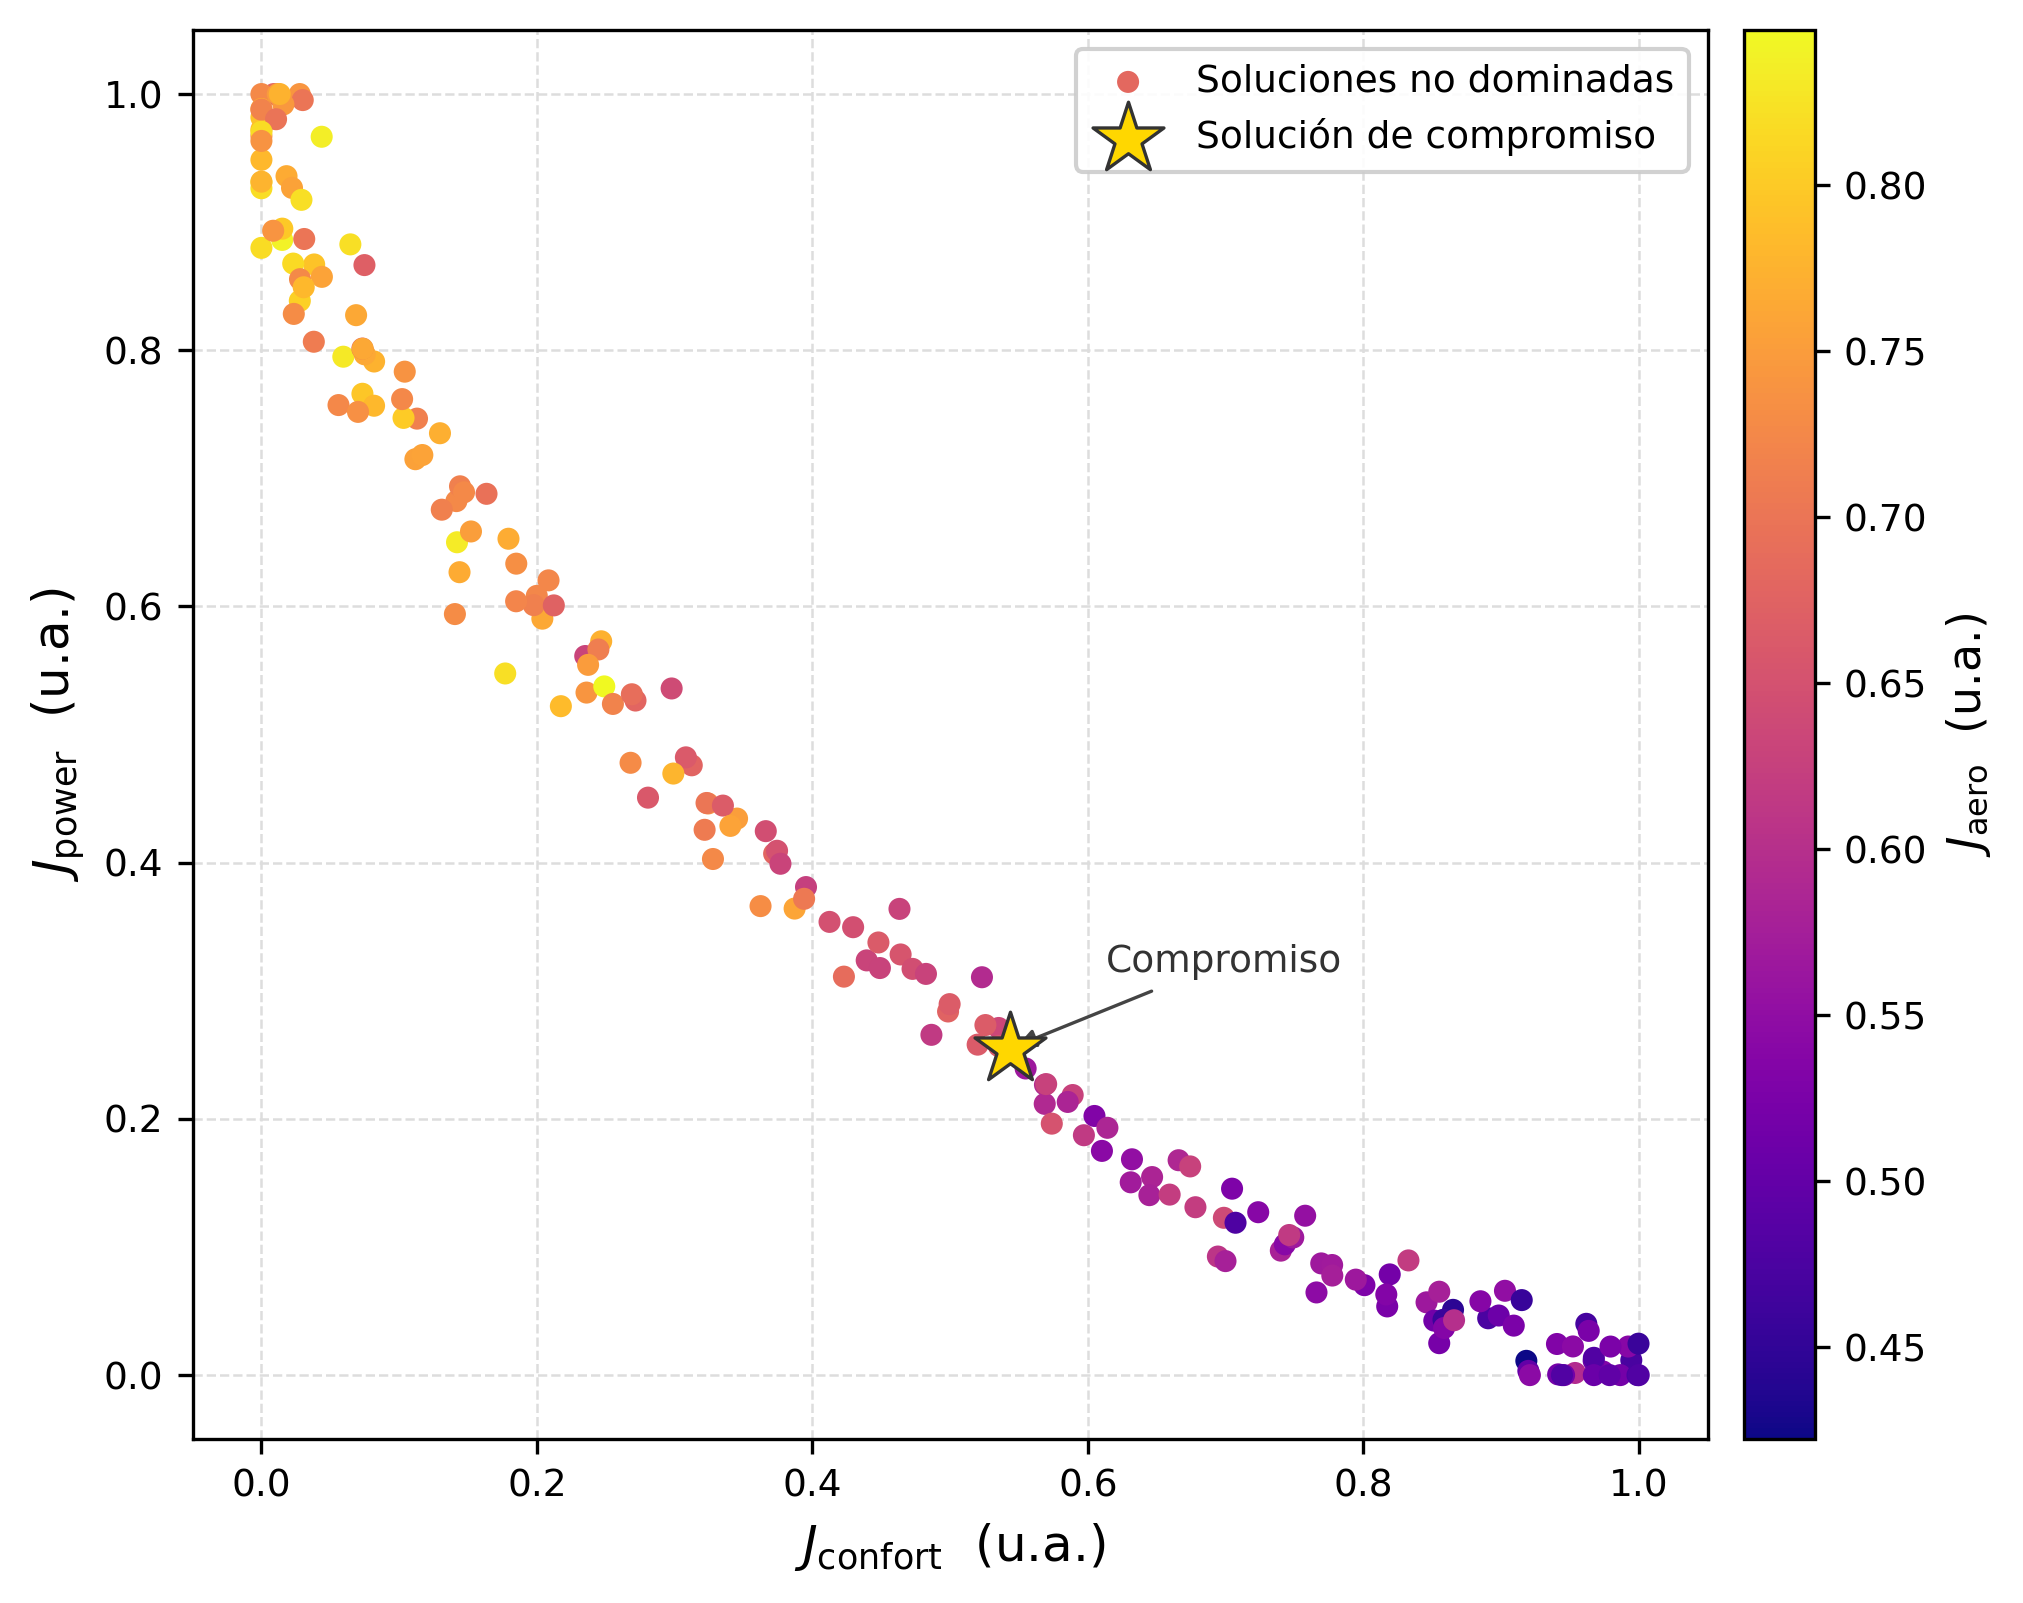
\includegraphics[width=\textwidth, height=0.74\textheight, keepaspectratio]{pareto_nsga2_2d.png}\\
            {\scriptsize Frente de Pareto 2D con mapa de calor de $J_\text{aero}$.}
        \end{column}
    \end{columns}
\end{frame}

% --- Validación postura (ang_act + ang_opt ambs CUADRADAS -> lado a lado 48%) ---
\begin{frame}{Validación cinemática: antes y después}
    \begin{columns}[c]
        \begin{column}{0.48\textwidth}
            \centering
            {\small\textbf{Configuración actual}}\\[4pt]
            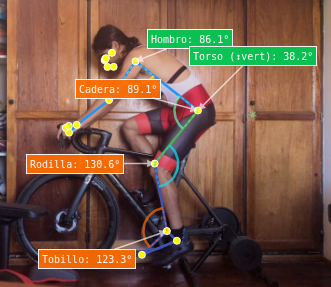
\includegraphics[width=0.92\textwidth]{ang_act.png}
        \end{column}
        \begin{column}{0.48\textwidth}
            \centering
            {\small\textbf{Configuración optimizada}}\\[4pt]
            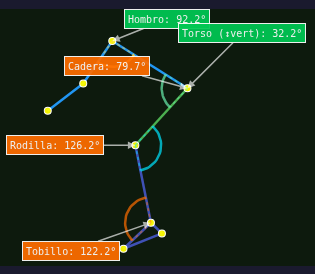
\includegraphics[width=0.92\textwidth]{ang_opt.png}
        \end{column}
    \end{columns}
    \vspace{4pt}
    \begin{center}
        \small
        Mayor inclinación de torso (aerodinámico) manteniendo
        la rodilla dentro del rango seguro ($\le 147^{\circ}$).
    \end{center}
\end{frame}

% --- Rodilla: rodilla.png ancho completo (2.97x) ---
\begin{frame}{Validación cinemática: ángulo de rodilla}
    \vspace{-4pt}
    \begin{center}
        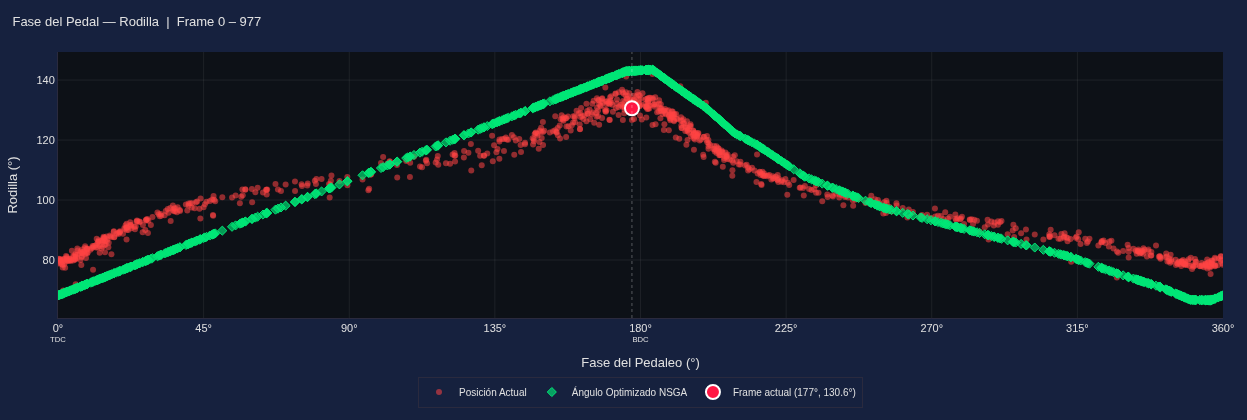
\includegraphics[width=\textwidth, height=0.80\textheight, keepaspectratio]{rodilla.png}
    \end{center}
    \vspace{-4pt}
    {\centering\scriptsize Ángulo articular de rodilla a lo largo del ciclo de pedaleo. La configuración optimizada mantiene el rango $70^{\circ}$--$147^{\circ}$ en toda la fase.\par}
\end{frame}

% --- Diagnóstico visual (optimizado.png 1.33x ANCHA -> imagen grande) ---
\begin{frame}{Diagnóstico visual aumentado}
    \begin{columns}[T]
        \begin{column}{0.38\textwidth}
            \small
            El pipeline genera un reporte visual que cierra el
            \textbf{lazo de control humano}:\\[4pt]
            marcadores articulares y ángulos articulares
            superpuestos sobre el fotograma de video.
        \end{column}
        \begin{column}{0.60\textwidth}
            \centering
            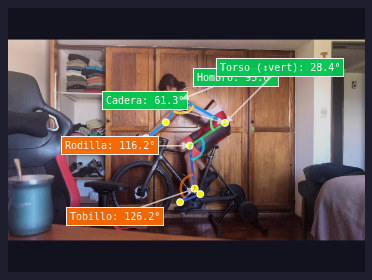
\includegraphics[width=\textwidth]{optimizado.png}\\
            {\scriptsize Postura optimizada con marcadores y ángulos superpuestos.}
        \end{column}
    \end{columns}
\end{frame}

% --- Recomendaciones (tabla, sin figura) ---
\begin{frame}{Recomendaciones de ajuste físico}
    \begin{center}
        \small
        \begin{tabular}{@{}lllc@{}}
            \toprule
            \rowcolor{fiubablue!20}
            \textbf{Componente} & \textbf{Parámetro} & \textbf{Magnitud} & \textbf{Dirección} \\
            \midrule
            Sillín   & Posición (\textit{fore/aft}) & 13,5\,mm & Hacia atrás \\
            Sillín   & Altura                        & 11,4\,mm & Subir       \\
            Manillar & Alcance (\textit{reach})       & 23,0\,mm & Acortar     \\
            Manillar & Altura (\textit{stack})        & 26,4\,mm & Bajar       \\
            \bottomrule
        \end{tabular}
    \end{center}
    \vspace{6pt}
    \begin{itemize}
        \item Reducción del \textit{reach}: compensa la potencia de 120\,mm instalada.
        \item Reducción del \textit{stack}: equivale a retirar 2 espaciadores físicos.
    \end{itemize}
\end{frame}

% ============================================================
\section{Cap. 5 -- Conclusiones y trabajo futuro}
% ============================================================

\begin{frame}{Conclusiones generales}
    \begin{itemize}
        \item Pipeline robusto: visión artificial + física mecánica + IA.
        \item Ruido de BlazePose mitigado con filtros cinemáticos y Kalman.
        \item \textbf{Democratización del \textit{bike fitting}:} resultados
              comparables a laboratorio sin marcadores ni instrumentos invasivos.
        \item Cumplimiento de requerimientos: \textbf{89\,\%}.
    \end{itemize}
    \vspace{4pt}
    \begin{block}{Aporte principal}
        Sistema accesible, reproducible y extensible para ajuste biomecánico
        dinámico asistido por IA.
    \end{block}
\end{frame}

\begin{frame}{Trabajo futuro}
    \begin{itemize}
        \item Sensores de potencia bilaterales (Garmin Rally RK\,200)
              para validar la dinámica inversa experimentalmente.
        \item Extender topología a extremidades superiores y hombros.
        \item Ampliar muestra de ciclistas (generalización demográfica).
        \item Despliegue en producción con soporte multiusuario y
              retroalimentación longitudinal.
    \end{itemize}
\end{frame}

\begin{frame}{Demostración en video}
    \begin{center}
        \href{https://drive.google.com/file/d/1xw4t4PQROlvFsohb3VDxOIq96WslJAHQ/view?usp=sharing}{%
            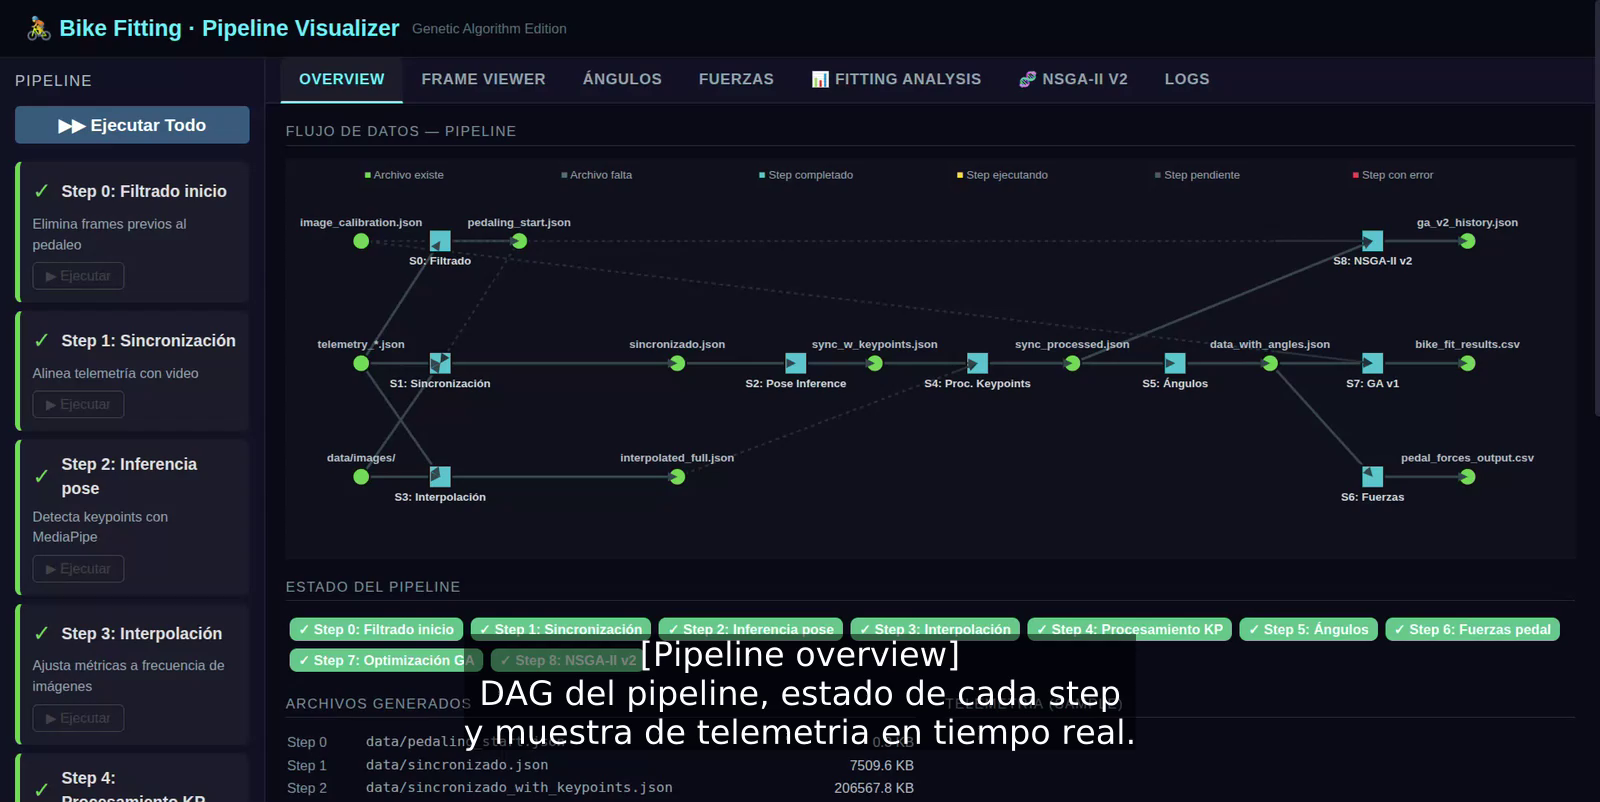
\includegraphics[width=0.82\textwidth,height=0.62\textheight,keepaspectratio]{genetics_bikefitting_demo_preview.png}%
        }\\[8pt]
        {\scriptsize Haga clic sobre la imagen para abrir el video en Google Drive.}\\[8pt]
        \href{https://drive.google.com/file/d/1xw4t4PQROlvFsohb3VDxOIq96WslJAHQ/view?usp=sharing}{\beamergotobutton{Ver video en Drive}}
    \end{center}
\end{frame}

% ============================================================
% CIERRE
% ============================================================
\begin{frame}[plain]
    \begin{center}
        \vspace{1.5cm}
        {\Huge \color{fiubablue} ¿Preguntas?} \\[1cm]
        {\Large ¡Muchas gracias!} \\[1.5cm]
        \footnotesize
        \textbf{Ing. Rodrigo Iván Goñi} \\
        FIUBA -- Carrera de Especialización en Inteligencia Artificial \\[6pt]
        \textbf{Director:} MSc. Fernando Corteggiano
    \end{center}
\end{frame}

\end{document}
